%%
%% adaptiveUnion.tex
%% 
%% Made by Jeremy Barbay
%% Login   <jbarbay@condorito>
%% 
%% Started on  Thu Apr 17 18:29:32 2008 Jeremy Barbay
%% Last update Thu Apr 17 18:29:32 2008 Jeremy Barbay
%%

\chapter{Set Operations}
\label{cha:adaptive-union}


\section{Introduction}
\label{sec:introduction}


\subsection{Relation with Merge Sort}
\label{sec:relation-with-merge}

We already talked about merging sorted arrays, in the context of
sorting algorithms based on partitioning.
%
The paper from Chen and
Carlsson~\cite{onPartitionsAndPresortednessOfSequences} explores more
this direction, where you can restrict the sizes of the arrays
considered through restrictions on the partitioning algorithm: the
goal is to balance the disorder inside each subarray and the
difference of sizes between subarrays.

\subsection{Disjonctive and Conjunctive queries}
\label{sec:disj-conj-quer}


Consider search engines where {\em queries} are composed of several
keywords, each one being associated with a sorted array of references
to entries in some database~\cite[p.~136]{gigabytes}.
%
The answer to a {\em conjunctive query} is the intersection of
the sorted arrays corresponding to each keyword.
%
Most search engines implement these queries.
%
The algorithms are in the {\em comparison model}, where comparisons
are the only operations permitted on references.


The merging of sorted array also occurs in other contexts, where the
arrays can be of any size, as for example when computing the union of
two sorted indexes, to answer a disjonctive query.
%
The problem over two arrays is identical to the problem of
intersecting the two sorted indexes, as for example to answer a
conjunctive query (aka Google like query).

One type of algorithms to compute the union or the intersection of
more than two arrays consists in computing their combination two by
two, up to the final result: implementations of relational data bases
routinely use this type of algorithms and optimize the order in which
the arrays are considered.



\subsection{Traditional Algorithms: Binary Merge}
\label{sec:trad-algor-binary}

\begin{algorithm}
  \begin{algorithmic}
    \WHILE{some elements are left}
    \IF{the two first elements are of equal value}
    \STATE{output their value}
    \STATE{skip them}
    \ELSE
    \STATE{search for the largest of the two elements $x$ in the array $B$ containing the smallest one}
    \STATE{skip all the elements smaller than $x$ in the array $B$}   \ENDIF
    \ENDWHILE
  \end{algorithmic}
\caption{Naive Merging Algorithm}
\end{algorithm}


There is an extensive literature on the
merging~\cite{optimalMergingOf2ElementsWithNElements,aSimpleAlgorithmForMergingTwoDisjointLinearlyOrderedSets,improvingTheBoundOnOptimalMerging,significantImprovementsToTheHwangLinMergingAlgorithm,twoProbabilisticResultsOnMerging,averageCaseAnalysisOfTheMergingAlgorithmOfHwangAndLin}
or intersection~\cite{aFastSetIntersectionAlgorithmForSortedSequences}
of two sorted arrays. 
%
The two problems are similar, as both require the algorithm to place
each element in the context of the other elements.
%
In relational databases, the intersection of more than two arrays is
computed by intersecting the arrays two by two.
%
The only optimization available in this context consist in choosing
the {\em order} in which those sets are intersected, and the
literature explores how to use statistics precomputed on the content
of the database to choose the best order~\cite[and its
references]{anOverviewOfQueryOptimizationInRelationalSystems}.


\subsection{Notations about Sets}
\label{sec:notations-about-sets}

We define  the {\em signature} of an instance.
%
\begin{definition}
We consider $\rm U$ to be a totally ordered space.
%
An {\em instance} is composed of $k$ sorted arrays $A_1,\ldots,A_k$ of
positive sizes $n_1,\ldots, n_k$ and composed of elements from
$\rm{U}$.
%
The {\em signature} of such an instance is $(k,n_1,\ldots,n_k)$.
%
An instance is ``of signature {\em at most}'' $(k,n_1,\ldots,n_k)$ if it
can be completed by adding arrays and elements to form an instance of
signature exactly $(k,n_1,\ldots,n_k)$.
\end{definition}
%
\begin{example}
Consider the instance of Figure~\ref{fig:instanceOne}, where the
ordered space is the set of positive integers: it has signature
$(7,1,4,4,4,4,4,4)$
%
\begin{figure}
$$
\begin{array}{c|c|c|c|c|c|c|c|c|c|c|c|c|c|c|c|c|c|c|c|c|c|c|c|c|c}\cline{2-2}
A=& \bf 9\\ \cline{2-5}
B=& 1& 2&\bf  9&11\\ \cline{2-5}
C=& 3&\bf  9&12&13\\ \cline{2-5}
D=&\bf  9&14&15&16\\ \cline{2-5}
E=& 4&\bf 10&17&18\\ \cline{2-5}
F=& 5& 6& 7&\bf 10\\ \cline{2-5}
G=& 8&\bf 10&19&20\\ \cline{2-5}
\end{array}
\hfill
\begin{array}{cccccccccccccccccccccccccc}
A:&  &  &  &  &  &  &  &  & 9&  &  &  &  &  &  &  &  &  &  &  \\
B:& 1& 2&  &  &  &  &  &  & 9&  &11&  &  &  &  &  &  &  &  &  \\
C:&  &  & 3&  &  &  &  &  & 9&  &  &12&13&  &  &  &  &  &  &  \\
D:&  &  &  &  &  &  &  &  & 9&  &  &  &  &14&15&16&  &  &  &  \\
E:&  &  &  & 4&  &  &  &  &  &10&  &  &  &  &  &  &17&18&  &  \\
F:&  &  &  &  & 5& 6& 7&  &  &10&  &  &  &  &  &  &  &  &  &  \\
G:&  &  &  &  &  &  &  & 8&  &10&  &  &  &  &  &  &  &  &19&20\\
\end{array}
$$ 
\caption{An instance of the intersection problem: on the left is the
array representation of the instance, on the right is a representation
which expresses in a better way the structure of the instance, where
the x-coordinate of each element is equal to its
value.}\label{fig:instanceOne}
\end{figure}
\end{example}
%

\section{$k$-Union}
\label{sec:k-union}

DLM\cite{dlm}

\section{$k$-Intersection}
\label{sec:k-intersection}

\begin{definition}
The {\em Intersection} of an instance is the set
$A_1\cap\ldots\cap A_k$ composed of the elements that are present in
$k$ distinct arrays.
\end{definition}
\begin{example}
The intersection $A\cap B\cap\ldots\cap G$ of the instance of
Figure~\ref{fig:instanceOne} is empty, as no element is present in
more than $4$ arrays.
\end{example}

Any algorithm (even a non-deterministic one) computing the
intersection must prove the correctness of the output: first, it must
certify that all the elements of the output are indeed elements of the
$k$ arrays; second, it must certify that no element of the
intersection has been omitted, by exhibiting some certificate that
there can be no other elements in the intersection than those output.
%
We define the partition-certificate as such a proof.
%
\begin{definition}
A {\em partition-certificate} is a partition $(I_j)_{j\leq\delta}$ of
$\rm U$ into intervals such that any singleton $\{x\}$ corresponds to
an element $x$ of $\cap_i A_i$, and each other interval $I$ has an
empty intersection $I\cap A_i$ with at least one array~$A_i$.
\end{definition}


\subsection{Gap}
\label{sec:gap}

DLM\cite{dlm}

\subsection{Alternation~\cite{alternationAndRedundancyAnalysisOfTheIntersectionProblem}}
\label{sec:alternation}





Imagine a function which indicates for each element $x\in\rm U$ the
name of an array not containing $x$ if $x$ is not in the intersection,
and ``all'' if $x$ is in the intersection.
%
The minimal number of times such a function {\em alternates} names,
for $x$ scanning $\rm U$ in increasing order, is just one less than
the minimal size of a partition-certificate of the instance, which is
called the {\em alternation} of the instance.
%
\begin{definition}\label{def:alternation}
The {\em alternation} $\delta$ of an instance
$(A_1,\ldots,A_k)$ is the minimal number of intervals forming a
partition-certificate of this instance.
\end{definition}
\begin{example}
The alternation of the instance in Figure~\ref{fig:instanceOne} is
$\delta{=}3$, as we can see on the right representation that the
partition $(-\infty,9),[9,10),[10,+\infty)$ is a partition-certificate
of size $3$, and that none can be smaller.
\end{example}

The alternation of an instance $I$ is also the complexity of the best
non-deterministic algorithm on $I$ (plus $1$), i.e. the {\em
non-deterministic complexity}.
%
This non-deterministic complexity forms a weak lower bound on the
complexity of any randomized or deterministic algorithm solving $I$,
and hence a natural measure of the difficulty of the instance.

\begin{theorem}[\ Alternation Upper Bound~\cite{adaptiveIntersectionAndTThresholdProblems}]\label{th:alternationUB} 
There is a deterministic algorithm which performs
$O(\delta\sum_{i=1}^k\log(n_i/\delta))$ comparisons on any instance of
signature $(k,n_1,\ldots,n_k)$ and alternation~$\delta$.
\end{theorem}
\begin{proof}
The deterministic version of Algorithm {\tt Rand Intersection} (see
Section~\ref{sec:algorithm}), where the choice of a random array is
replaced by the choice of the next array in a fixed order, performs
$O(\delta\sum_{i=1}^k\log(n_i/\delta))$ comparisons on an instance of
signature $(k,n_1,\ldots,n_k)$ and of alternation $\delta$.
%
Its analysis is very similar to the one of the randomized version
given in the proof of Theorem~\ref{th:redundancyUB}.

Note that this algorithm is distinct from the algorithm presented
previously~\cite{adaptiveIntersectionAndTThresholdProblems}, where the algorithm was performing
unbounded searches in parallel in the arrays. 
%
Here the algorithm performs one unbounded search at a time, which
saves some comparisons in  many cases,
for any arbitrary signature $(k,n_1,\ldots,n_k)$ (but not
in the worst case).  \qed \end{proof}

The lower bound apply to any randomized algorithm, when a mere
deterministic algorithm is optimal.
%
Does it mean that no randomized algorithms can do better than a
deterministic one on the intersection problem?
%
We refine the analysis to answer this question.




\subsection{Redundancy~\cite{optimalityOfRandomizedAlgorithmsForTheIntersectionProblem,alternationAndRedundancyAnalysisOfTheIntersectionProblem}}
\label{sec:redundancy}





By definition of the partition-certificate:
\begin{itemize}
\item for each singleton $\{x\}$ of the partition, any algorithm must
find the position of $x$ in all arrays $A_i$, which takes $k$ searches;
\item for each interval $I_j$ of the partition, any algorithm must
find an array, or a set of arrays, such that the intersection of $I_j$
with this array, or with the intersection of those arrays, is empty.
\end{itemize}
%
The cost for finding such a set of arrays can vary, and depends on the
choices performed by the algorithm.
%
In general, it requires fewer searches if there are many possible
answers.
%
To take this into account, for each interval $I_j$ of the
partition-certificate we will count the number $r_j$ of arrays whose
intersection with $I_j$ is empty.
%
The smaller is $r_j$, the harder is the instance: $1/r_j$ measures
the contribution of this interval to the difficulty of the instance.
%
\begin{example}
Consider for instance the interval $I_j=[10,11)$ in the instance of
Figure~\ref{fig:instanceOne}: $r_j=4$ arrays have an empty
intersection with it.
%
A randomized algorithm, choosing an array uniformly at random, has
probability $r_j/k$ to find an array which does not intersect $I_j$,
and will do so after at most $\lceil k/r_j\rceil$ trials on average,
even if it tries several times in the
same array because it doesn't memorize which array it tried before.
%
As the number of arrays $k$ is fixed, 
the value $1/r_j$ measures the difficulty of proving that no element
of $I_j$ is in the intersection of the instance.
\end{example}
%
We name the sum of those contributions the {\em redundancy} of the
instance, and it forms our new measure of difficulty:
%
\begin{definition} \label{def:redundancy}
Let $A_1,\ldots,A_k$ be $k$ sorted arrays, 
and let $(I_j)_{j\leq\delta}$ be a partition-certificate for this instance.
\begin{itemize}
\item The {\em redundancy $\rho(I)$ of an interval or singleton $I$} is defined as 
equal to $1$ if $I$ is a singleton, and equal to $1/\#\{i,\,A_i\cap I=\emptyset\}$ otherwise.
\item The {\em redundancy $\rho((I_j)_{j\leq\delta})$ of a
partition-certificate} $(I_j)_{j\leq\delta}$ is the sum $\sum_j
\rho(I_j)$ of the redundancies of the intervals composing it.
\item The {\em redundancy $\rho\left( (A_i)_{i\leq k}\right)$ of an
instance} of the intersection problem is the minimal redundancy $\min
\{ \rho\left((I_j)_{j\leq\delta}\right),\, \forall (I_j)_{j\leq\delta}
\}$ of a partition-certificate of the instance.
\end{itemize}
\end{definition}

Note that the redundancy is always well defined and finite: if $I$ is
not a singleton then by definition there is at least one array $A_i$
whose intersection with $I$ is empty, hence
$\#\{i,\,A_i\cap I=\emptyset\}>0$.
%
\begin{example}
The partition-certificate
$\{(-\infty,9),[9,10),[10,11),[11,+\infty)\}$ has redundancy at most
${1/2}{+}{1/3}{+}{1/4}{+}{1/2} = {7/6}$ for the
instance given Figure~\ref{fig:instanceOne}, and no other
partition-certificate has a smaller redundancy, hence the instance has
redundancy ${7/6}$.
\end{example}

The main idea is that the redundancy analysis permits to measure the
difficulty of the instance in a finer way than the alternation
analysis: for fixed $k,n_1,\ldots,n_k$ and $\delta$, several instances
of signature $(k,n_1,\ldots,n_k)$ and alternation $\delta$ may present
various levels of difficulty, and the redundancy helps to distinguish
between those.
%
\begin{example}
In the instance from Figure~\ref{fig:instanceOne}, the only way to
prove the emptiness of the intersection is to compute the intersection
of one of the arrays chosen from $\{A,B,C,D\}$ with one of the arrays
chosen from $\{E,F,G\}$, because $9\in A\cap B\cap C\cap D$ and $10\in
E\cap F\cap G$.
%
For simplicity, and without loss of generality, suppose that the
algorithm searches to intersect $A$ with another array in
$\{B,C,D,E,F,G\}$, and consider the number of unbounded searches
performed, instead of the number of comparisons.
%
The randomized algorithm looking for the element of $A$ in a random
array from $\{B,C,D,E,F,G\}$ performs on average only $2$ searches, as
the probability to find an array whose intersection is empty with $A$
is then $1/2$.

On the other hand, consider the instance of
Figure~\ref{fig:instanceTwo}, a variant of the instance of
Figure~\ref{fig:instanceOne}, where element $9$ is present in all the
arrays but $E$.
%
As the two instances have the same signature and alternation, the
alternation analysis yields the same lower bound for both instances.
%
But the randomized algorithm described above now performs on average
$k/2$ searches, as opposed to $2$ searches on the original instance.
%
This difference in difficulty, between those very similar instances,
is not expressed by a difference of alternation, but it is expressed
by a difference of redundancy: the new instance has a redundancy of
${1/2}{+}1{+}{1/6}{+}{1/2}=2{+}{1/6}$, which is {\em
larger} by one than the redundancy ${7/6}$ of the original
instance.
%
This difference of one corresponds to $k$ more doubling searches for
this simple instance.
%
This difference is used in Section~\ref{sec:comparison} to create
instances where a deterministic algorithm performs $O(k)$ times more
searches and comparisons than a randomized algorithm.
\end{example}

\begin{figure}
$$
\begin{array}{c|c|c|c|c|c|c|c|c|c|c|c|c|c|c|c|c|c|c|c|c|c|c|c|c|c}\cline{2-2}
A=& \bf 9\\ \cline{2-5}
B=& 1& 2&\bf  9&11\\ \cline{2-5}
C=& 3&\bf  9&12&13\\ \cline{2-5}
D=&\bf  9&14&15&16\\ \cline{2-5}
E=& 4&\bf 10&17&18\\ \cline{2-5}
F=& 5& 6& 7&\bf 9\\ \cline{2-5}
G=& 8&\bf 9&19&20\\ \cline{2-5}
\end{array}
\hfill
\begin{array}{cccccccccccccccccccccccccc}
A:&  &  &  &  &  &  &  &  & 9&  &  &  &  &  &  &  &  &  &  &  \\
B:& 1& 2&  &  &  &  &  &  & 9&  &11&  &  &  &  &  &  &  &  &  \\
C:&  &  & 3&  &  &  &  &  & 9&  &  &12&13&  &  &  &  &  &  &  \\
D:&  &  &  &  &  &  &  &  & 9&  &  &  &  &14&15&16&  &  &  &  \\
E:&  &  &  & 4&  &  &  &  &  &10&  &  &  &  &  &  &17&18&  &  \\
F:&  &  &  &  & 5& 6& 7&  & 9&  &  &  &  &  &  &  &  &  &  &  \\
G:&  &  &  &  &  &  &  & 8& 9&  &  &  &  &  &  &  &  &  &19&20\\
\end{array}
$$ 
\caption{A much more difficult variant of the instance of
Figure~\ref{fig:instanceOne}: only two elements changed, $F[4]$ and
$G[2]$ which were equal to $10$ and are now equal to $9$, but the
redundancy is now
$\rho={1/2}{+}1{+}{1/6}{+}{1/2}=2{+}{1/6}$.
}\label{fig:instanceTwo}
\end{figure}



%\subsection{Randomized algorithm}\label{sec:algorithm}


For simplicity, we assume that all arrays contain the element
$-\infty$ at position $0$ and the element $+\infty$ at position
$n_i{+}1$.
%
Given this convention, the intersection algorithm can ignore the sizes
of the sets.
%
This is the case in particular in pipe-lined computations, where the
sets are not completely computed when the intersection starts, for
instance in parallel applications.



An {\tt unbounded search} looks for an element $x$ in a sorted array
$A$ of unknown size, starting at position $init$.
%
It returns a value $p$ such that $A[p-1]{<}x{\leq}A[p]$, called the
{\em insertion rank} of $x$ in $A$.
%
It can be performed combining the doubling search and binary search
algorithms~\cite{adaptiveIntersectionAndTThresholdProblems,dlm,dlmAlenex},
and is then of complexity $2\lceil\log_2(p{-}init)\rceil$, or in a
more complicated
way~\cite{anAlmostOptimalAlgorithmForUnboundedSearching} to improve
the complexity by a constant factor of less than $2$.


 
Using unbounded search rather than binary search is crucial to the
complexity of the intersection algorithm.
%
Consider the task of searching $d$ elements $x_1\leq x_2 \leq \ldots
\leq x_d$ in a sorted array of size $n$.
%
It requires $d\log n_i$ comparisons using binary search, but less than
$2d\log(n_i/d)$ comparisons using unbounded search.
%
To see that, define $p_j$ such that $p_0=0$ and $A[p_j]=x_j\,\forall
j\in\{1,\ldots,d\}$: the $j$th doubling search performs, no more than
$2\log(p_j-p_{j-1})$ comparisons.
%
By concavity of the log, the sums
$\sum_{j\leq d}2\log(p_j-p_{j-1})$ is no larger than
$2d\log(\sum_{j\leq d}(p_j-p_{j-1})/d)$.
%
The sum $\sum_{j\leq d}(p_j-p_{j-1})$ is equal to $p_d-p_0$, which is
smaller than the size $n$ of the array.
%
Hence the $d$ doubling searches perform less than $2d\log(n_i/d)$
comparisons.




\begin{theorem}\label{th:correctnessAlgorithm}
Algorithm {\tt Rand Intersection}
(see Fig.~\ref{fig:randIntersection}) computes the intersection of
the arrays given as input.
\end{theorem}

%
\def\R{\hbox{\tt Result}}

\begin{figure}
\hrule
\vspace{3pt}
{\bf Algorithm} {\tt Rand Intersection $(A_1,\ldots,A_k)$}
\vspace{3pt}
\hrule

\begin{tabular*}{1cm}{lll}
\multicolumn{3}{l}{{\bf for all} $i$ {\bf do} $p_i\leftarrow 1$ {\bf end for}} \\
\multicolumn{3}{l}{$\R\leftarrow \emptyset$; $s\leftarrow 1$} \\
\multicolumn{3}{l}{\bf repeat} \\
&\multicolumn{2}{l}{   $m \leftarrow A_s[p_s]$} \\
&\multicolumn{2}{l}{   $\#{\hbox{\tt NO}}\leftarrow 0$; $\#{\hbox{\tt YES}}\leftarrow 1$;}\\
&\multicolumn{2}{l}{ {\bf while} {${\hbox{\tt YES}} < k$  and  $\#{\hbox{\tt NO}}=0$} }\\
&&     Let $A_s$ be a random array s.t. $A_s[p_s]\neq m$.\\
&&     $p_s \leftarrow$ {\tt Unbounded Search}$(m,A_s,p_s)$ \\
&&     {\bf if }{$A_s[p_s]\neq m$} 
      {\bf then } $\#{\hbox{\tt NO}}\leftarrow 1$
      {\bf else }  $\#{\hbox{\tt YES}}\leftarrow{\hbox{\tt YES}}+1$ {\bf end if} \\
& \multicolumn{2}{l}{\bf endwhile} \\
& \multicolumn{2}{l}{{\bf if }{$\#{\hbox{\tt YES}} =k$ } {\bf then } $\R\leftarrow \R\cup \{ m \}$ {\bf end if} }\\
& \multicolumn{2}{l}{{\bf for all} $i$ such that $A_i[p_i]=m$ {\bf do} $p_i \leftarrow p_i+1$   {\bf end for} }\\
\multicolumn{3}{l}{\bf until $m=+\infty$} \\
\multicolumn{3}{l}{{\bf return } $\R$} \\
\end{tabular*}
\hrule
\caption{The algorithm {\tt Rand Intersection}: 
Given $k$ non-empty sorted sets $A_1,\ldots,A_k$ of sizes
$n_1,\ldots,n_k$,
%
the algorithm computes in variable $\R$ the intersection
$A_1\cap\ldots\cap A_k$.
%
Note that the only random instruction is the choice of the array in
the inner loop.
%
}
\label{fig:randIntersection}

\end{figure}


\begin{proof}
Given $k$ non-empty sorted sets $A_1,\ldots,A_k$ of sizes
$n_1,\ldots,n_k$, the {\tt Rand Intersection} algorithm
(Fig.~\ref{fig:randIntersection}) computes the intersection
$A_1{\cap}\ldots{\cap} A_k$.
%
The algorithm is composed of two nested loops.
%
The outer loop iterates through potential elements of the intersection
in variable $m$ and in increasing order, and the inner loop checks for
each value of $m$ if it is in the intersection.

In each pass of the inner loop, the algorithm searches for $m$ in one
array $A_s$ which potentially contains it.
%
The invariant of the inner loop is that, at the start of each pass and
for each array $A_i$, $p_i$ denotes the first potential position for
$m$ in $A_i$: $A_i[p_i-1]<m$.
%
The variables $\#{\hbox{\tt YES}}$ and $\#{\hbox{\tt NO}}$ count how
many arrays are known to contain $m$, and are updated depending on the
result of each search.

A new value for $m$ is chosen every time we enter the outer loop, at
which time the current subproblem is to compute the intersection on the
sub-arrays $A_i[p_i,\ldots,n_i]$ for all values of $i$.
%
Any first element $A_i[p_i]$ of a sub-array could be a candidate, but
a better candidate is one which is larger than the last value of $m$:
%
the algorithm chooses $A_s[p_s]$, which is by definition larger than
$m$.
%
Then only one array $A_s$ is known to contain $m$, hence
$\#{\hbox{\tt YES}}\leftarrow 1$, and no array is known {\em not to} contain it,
hence $\#{\hbox{\tt NO}}\leftarrow 0$.
%
The algorithm terminates when all the values of the current array have
been considered, and $m$ has taken the last value $+\infty$.
\qed\end{proof}


We now analyze the complexity of Algorithm~{\tt Rand Intersection}
(Fig.~\ref{fig:randIntersection}) as a function of the redundancy
$\rho$ of the instance.
%
To understand the intuition behind the analysis, consider the
following example:
%
\begin{example}  

  For a fixed interval $I_j$, suppose that the algorithm receives six
  arrays such that $A_1$, $A_2$, $A_3$ and $A_4$ contain many elements
  from $I_j$ but have none in common, and such that $A_5$ and $A_6$ contain no
  elements from $I_j$.
  % 
  Ignore all steps of the algorithm where $m$ takes values out of the
  interval $I_j$: the interval defines a {\em phase} of the algorithm.
  % 
  Suppose that $m$ takes a value in $I_j$ at some point, for instance
  from $A_1$.
  % 
  At each iteration of the external loop, the algorithm ignores the
  array from which the current value of $m$ was taken, chooses one
  between the four remaining arrays, searches in the chosen one, and
  updates the value of $m$ accordingly.
  % 
  \begin{itemize}
  \item With probability $3/5$ the algorithm chooses the set $A_1$,
    $A_2$, $A_3$ or $A_4$ (depending of which set the current value of
    $m$ comes from) and potentially fails to terminate the phase.
  \item With probability $2/5$ the algorithm chooses $A_5$ or $A_6$,
    performs a search in it (there might be elements left from
    intervals $I_1\cup\ldots\cup I_{j-1}$), and updates $m$ to a value
    from $I_{j+1}$, which terminates the current phase.
  \end{itemize}

  We are interested in the number $C_i^j$ of searches performed in
  each array $A_i$ during this phase.
  % 
  As $m$ takes a value outside of $I_j$ after a search in $A_5$ or
  $A_6$, $C_5^j$ and $C_6^j$ are random boolean variables, which
  depend only on the last choice of the algorithm before
  changing phase: the expectation of $C_5^j$ (resp. $C_6^j$) is
  exactly the probability that $A_5$ (resp. $A_6$) is picked knowing
  that one of those is picked, i.e. $1/2$.

  The algorithm can perform many searches in $A_1$, $A_2$, $A_3$ and
  $A_4$, so the variables $C_1^j$, $C_2^j$, $C_3^j$ and $C_4^j$ are
  random integer variables, which depend on all the choices of the
  algorithm but the last.
  % 
  The probability that $A_1$ is chosen is null if $m$ comes from $A_1$.
  % 
  Otherwise it is less than the probability that $A_1$ is chosen
  knowing that $m$ doesn't come from $A_1$: $\Pr[A_1$ is chosen
  $] = \Pr[A_1$ is chosen and $m$ does not come from $A_1]$
  $\leq \Pr[A_1$ is chosen $ | m $ does not come from
    $A_1].$
  % 
  Hence the probability that $A_1$ is chosen is less than $1/4$.
  
  $C_1^j$ is increased each time $A_1$ is chosen (probability $a\leq
  1/5$), is finalized as soon as $A_5$ or $A_6$ is chosen (probability
  $b=2/5$), and stays the same each time another array is chosen
  (probability $c\geq 2/5$).
  % 
  Ignore all the steps where $C_2^j$, $C_3^j$ or $C_4^j$ are
  increased:
  % 
  knowing that $C_2^j$, $C_3^j$ or $C_4^j$ are not increased, the
  probability that $C_1^j$ is increased is $a/(a+b)\leq 1/3$, and the
  probability that it is finalized is $b/(a+b)\geq 2/3$.
  % 
  Such a system will iterate at most $3/2$ times on average, and
  increment $C_1^j$ each time but the last, i.e. $3/2-1=1/2$ times on
  average.
  % 
  The same reasoning holds for $A_2$, $A_3$ and $A_4$.
  % 
  Hence in this example $E(C_i^j)=1/2$ for each set $A_i$, where $2$
  is the number of arrays which contain no elements from $I_j$.
\end{example}
The proof of Theorem~\ref{th:redundancyUB} argues similarly in the
more general case.



\begin{theorem}[Redundancy Upper Bound~\cite{optimalityOfRandomizedAlgorithmsForTheIntersectionProblem}]\label{th:redundancyUB}
Algorithm {\tt Rand Intersection}
(Fig.~\ref{fig:randIntersection}) performs on average
$O(\rho\sum_{i=1}^k\log(n_i/\rho))$ comparisons on any instance of signature
$(k,n_1,\ldots,n_k)$ and of redundancy $\rho$.
\end{theorem}

\begin{proof}
Let $(I_j)_{j\leq \delta}$ be a partition-certificate of minimal
redundancy $\rho$.
%
Each comparison performed by the algorithm is said to be performed in
{\em phase $j$} if $m\in I_j$ for some interval $I_j$ of the
partition.
%
Let $C_i^j$ be the number of searches performed by the algorithm
during phase $j$ in array $A_i$,
%
let $C_i=\sum_j C_i^j$ be the number of searches performed by the algorithm in
 array $A_i$ over the whole execution,
%
and let $(r_j)_{j\leq\delta}$ be such that $r_j$ is equal to $1$ if
$I_j$ is a singleton, and to $\#\{i,\,A_i\cap I_j=\emptyset\}$
otherwise.


%%%% E(C_i) 

Let us consider a fixed phase $j\in\{1,\ldots,\delta\}$, and
compute the average number of searches $E(C_i^j)$ performed in each
array $A_i$ during phase $j$.
%
At each iteration of the internal loop, the algorithm chooses an array
in which $m$ is not known to be.
%
As $m$ always comes from one array, there are at most $k-1$ of those
arrays, hence each array is chosen with probability at least
$1/(k-1)$.
%
If the element $m$ currently considered is in the intersection, 
then each array $A_i$ will be searched and $C_i^j$ is equal to $1$.
%
In this case $1/r_j$ is also equal to $1$, so that
$C_i^j{=}1/r_j{=}E(C_i^j)$.

Suppose that $m$ is {\em not} in the intersection, and that $A_i\cap
I_j$ is empty.
%
Either $A_i$ is never chosen, and $C_i^j=0$; or $A_i$ is chosen, and
$C_i^j=1$, because the algorithm will terminate the phase after
searching in $A_i$.
%
The probability that $A_i$ is chosen is at most the probability that
it is chosen knowing that this is the last search of the phase:
$$\Pr[A_i\mbox{ is chosen}]  = \Pr[A_i\mbox{ is chosen and last search}]
\leq \Pr[A_i\mbox{ is chosen} | \mbox{ last search}].$$	      

As the arrays are chosen uniformly, this probability is
$\Pr\{C_i^j=1\}\leq{1/r_j}$, and the average number of searches is at
most $E(C_i^j)=1*\Pr\{C_i^j=1\}\leq{1/r_j}$.


The interesting case is when $m$ is not in the intersection but
$A_i\cap I_j\neq\emptyset$.
%
At each new search, either 
\begin{enumerate}
\item $C_i^j$ is incremented by one because the search occurred in
  $A_i$, which occurs with probability less than ${1/(k-1)}$;
%
\item or $C_i^j$ is fixed in a final way because an array was found
  which intersection with $I_j$ is empty, which occurs with
  probability ${r_j/(k-1)}$;
%
\item or $C_i^j$ is neither incremented nor fixed, if another array
  was searched but its intersection with $I_j$ is not empty.
  % 
\end{enumerate}
% 
The combined probability of the first and second case is
$1/(k-1)+r_j/(k-1)$.
%
Ignoring the third case where $C_i^j$ never changes, the conditional
probability of the first case is
$\frac{1}{k-1}/(\frac{1}{k-1}+\frac{r_j}{k-1})$.
%
Hence this system is equivalent to a system where $C_i^j$ is
incremented by one with probability at least $1/(1+r_j)$,
% 
and fixed with the remaining probability, at most ${r_j/(1+r_j)}$.
%
Such a system iterates at most $(1+r_j)/r_j$ times on average, and
increments $C_i^j$ at each iteration but the last: the final value
of $C_i^j$ is at most $(1+r_j)/r_j-1=1/r_j$.

    Hence the average number of searches performed in each array~$A_i$
    during phase~$j$ is $E(C_i^j)\leq 1/r_j$.
%
    Summing over all phases, it implies that the algorithm performs on
    average $E(C_i)\leq\sum_j {1/r_j}=\rho$ searches in each array
    $A_i$.



    %%% Nb Cmps in A_i for given C_i
    Let $g_{i,j}^\ell$ be the increment of $p_i$ due to the $\ell$th
    unbounded search in array $A_i$ during phase $j$.
%
    Notice that $\sum_{j,\ell}g_{i,j}^\ell \leq n_i$.
%
    The algorithm performs at most $2\log(g_{i,j}^\ell+1)$ comparisons
    during the $\ell$th search of phase $j$ in array $A_i$.
%
    So it performs at most $2\sum_{j,\ell}\log(g_{i,j}^\ell+1)$
    comparisons between $m$ and an element of array $A_i$ during the
    whole execution.
%
    Because of the concavity of the function $\log(x+1)$, this is
    smaller than $2C_i\log(\sum_{j,\ell}{g_{i,j}^\ell/C_i}+1)$, and
    because of the preceding remark
    $\left(\sum_{j,\ell}g_{i,j}^\ell{\leq}n_i\right)$, this is smaller
    than $2C_i\log({n_i/C_i}+1)$.


    %%% Average number of comparisons
    The functions $f_i(x){=}2x\log({n_i/x}{+}1)$ are concave for
    $x{\leq}n_i$, so $E(f_i(C_i)){\leq}f_i(E(C_i))$.
    % (see appendix~\ref{appendix:concavityfi})
%
    As the average complexity of the algorithm in array $A_i$ is
    $E(f(C_i))$, and as $E(C_i)=\rho$, on average the algorithm
    performs less than $2\rho\log({n_i/\rho}+1)$ comparisons between
    $m$ and an element in array $A_i$.
%
    Summing over $i$ we get the final result, which is
    $O(\rho\sum_i\log{n_i/\rho}).$ \qed\end{proof}



\subsection{Randomized Complexity Lower Bound(s)}\label{sec:lowerbound}

We prove now that lower bounds for the three analysis for
$(k,n_1,\ldots,n_k)$ fixed.
%
The proof is quite similar to the lower bound of the alternation
analysis~\cite{adaptiveIntersectionAndTThresholdProblems}, and differs
mostly in Lemma~\ref{lem:elementproblem}, which must be adapted to
each analysis.
%
The Lemmas~\ref{lem:elementproblem} and~\ref{lem:generaldistribution}
are used to prove the alternation lower bound in
Theorem~\ref{th:alternationLB} and to prove the redundancy lower bound
in Theorem~\ref{th:redundancyLB}.


\subsubsection{Core of the Lower Bound Proof}
\label{sec:core-lower-bound}

In {Lemma~\ref{lem:elementproblem}} we prove a lower bound on average
on a distribution of instances of alternation
and redundancy at most $\rho=4$ and of intersection size at
most $1$.
%
We use this result in {Lemma~\ref{lem:generaldistribution}} to define
a distribution on instances of alternation and
redundancy at most $\rho\in\{4,4n_1\}$ by combining $p=\theta(\rho)$
sub-instances.
%
Applying the Yao-von Neumann
principle~\cite{vonneumann1944,sion58,yao} in {
Theorem~\ref{th:standalonelowerbound}} gives us a lower bound of
$\Omega(\rho\sum_{i=2}^k\log(n_i/\rho))$ on the complexity of any
randomized algorithm for the intersection problem.


Finally in {Lemma~\ref{lem:rhoupperbound}}, we prove that any instance
of signature $(k,n_1,\ldots,n_k)$ has redundancy $\rho$ at most
$2n_1+1$, so that the redundancy analysis of
Theorem~\ref{th:standalonelowerbound} covers totally all instances for
a given signature $(k,n_1,\ldots,n_k)$.





\begin{lemma}\label{lem:elementproblem}
For any $k\geq 2$, $0{<}n_1{\leq}\ldots{\leq}n_k$, there is a
distribution on instances of the intersection problem with signature
at most $(k,n_1,\ldots,n_k)$, alternation and redundancy at most~$4$,
such that any deterministic algorithm performs at least
${(1/4)}\sum_{i=2}^k\log(2n_i+1)+\sum_{i=2}^k{1/(2n_i{+}1)}-k{+}2$
comparisons on average.
\end{lemma}
\begin{proof}
Let $C$ be the total number of comparisons performed by the algorithm,
and for each array $A_i$ note $F_i=\log_2(2n_i+1)$, and $F=\sum_{i=2}^k F_i$.

Let us draw an index $w\in\{2,\ldots,k\}$ equal to $i$ with probability
${F_i/F}$,
% ${\log n_i / (\sum_{l=2}^k \log n_l)}$;
%
and $(k-1)$ positions $(p_i)_{i\in\{2,\ldots,k\}}$ such that $\forall i$
each $p_i$ is chosen uniformly at random in $\{1,\ldots,n_i\}$.
%
Let $P$ and $N$ be two instances such that
%
 in both $P$ and $N$, for any $1{<}i{<}j{\leq}k$, $a{\in}A_1$, 
$b,c{\in}A_i$ and $d,e{\in}A_j$ then  $b{<}A_i[p_i]{<}c$ and $d{<}A_j[p_j]{<}e$ imply 
$b{<}d{<}a{<}c{<}e$ (see Figure~\ref{fig:PandNdistribution});
%
in $P$, $A_{w}[p_{w}]{=}A_1[1]$; 
%
in $N$ $A_{w}[p_{w}]{>}A_1[1]$;
%
and such that the elements at position $p_i$ in all other arrays
than $A_w$ are equal to $A_1[1]$.

\begin{figure}
\centerline{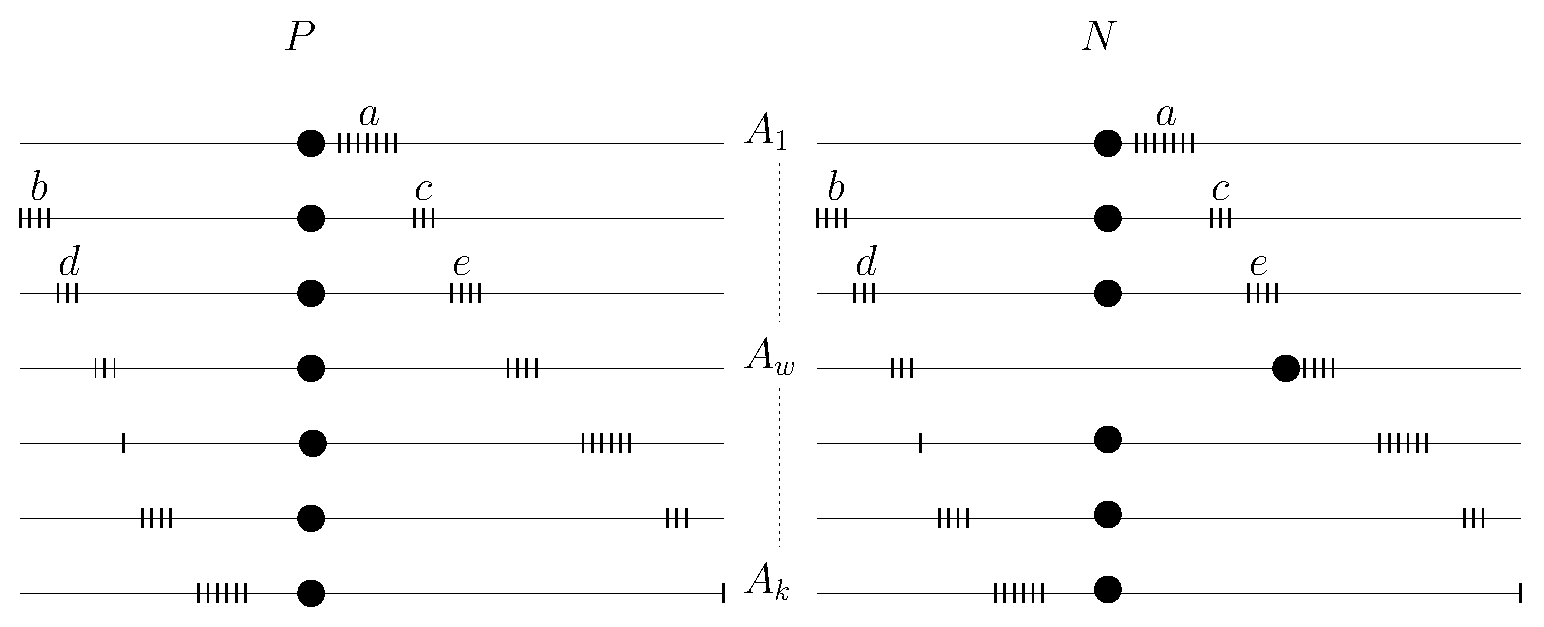
\includegraphics[angle=0,width=12cm]{PNdistribution.eps}}
\caption{Distribution on $(P,N)$: each element of value $v$ is
represented by a dot of x-coordinate $v$, and large dots correspond to
the element at position $p_i$ in each array
$A_i$. \label{fig:PandNdistribution}}
\end{figure}

Let $x=A_1[1]$ be the first element of the first array.
%
Define $x$-comparisons to be the comparisons between any element and $x$.
%
Because of the special relative positions of the elements, a
comparison between two elements $b$ and $d$ in any arrays does not
yield more information than the two comparisons between $x$ and $b$
and between $x$ and $d$: the positions of elements $b$ and $d$
relative to $x$ permit to deduce their order.
%
Hence any algorithm performing $C$ comparisons between arbitrary
elements can be expressed as an algorithm performing no more than $2C$
$x$-comparisons, and any lower bound $L$ on the complexity of
algorithms using only $x$-comparisons is an $L/2$ lower bound on the
complexity of algorithms using comparisons between arbitrary elements.

The alternation of such instances is at most $4$, and the redundancy
of such instances is no more than $3+{1/(k{-}1)}$, which is less
than $4$:
%
\begin{itemize}
\item the interval $\left(-\infty,A_{1}[1]\right)$ is sufficient to
  certify that no element smaller than $x$ is in the intersection, and
  stands for a redundancy of at most $1$;
%
\item the interval $\left(A_{1}[n_1],+\infty,\right)$ is sufficient to
  certify that no element larger than $A_{1}[n_1]$ is in the
  intersection, and stands for a redundancy of at most $1$;
%
\item  the interval $\left[A_1[1],A_{1}[n_{1}]\right]$ is sufficient in $N$
to complete the partition-certificate, and stands for a redundancy of
at most $1$;
% 
\item  the singleton $\{x\}$ and the interval
$\left(A_1[1],A_{1}[n_{1}]\right]$ are sufficient in $P$ to complete
the partition-certificate, and stand for a redundancy of at most
$1{+}{1/(k-1)}$.
\end{itemize}

The only difference between instances $P$ and $N$ is the relative
position of the element $A_{w}[p_{w}]$ to the other elements composing
the instance, as described in Figure~\ref{fig:PandNdistribution}.
%
Any algorithm computing the intersection of $P$ has to find the
$(k-1)$ positions $\{p_2,\ldots,p_k\}$.
%
Any algorithm computing the intersection of $N$ has to find $w$ and
the
associated
position $p_w$.
%
Any algorithm distinguishing between $P$ and $N$ has to find $p_w$:
%
we will prove that it needs on average almost
${F/2}={(1/2)}\sum_{i=2}^k\log_2(2n_i+1)$ $x$-comparisons to do so on
a distribution corresponding to the uniform choice between an instance
$N$ and an instance $P$.

Consider a deterministic algorithm using
only $x$-comparisons to compute the intersection.
%
As the algorithm  has not distinguished between $P$ and $N$ till it
found $w$, let $X_i$ denote the number of $x$-comparisons performed
 in array $A_i$ for both $P$ or $N$.
%
Let $Y_i$ denote the number of $x$-comparisons performed  in
array $A_i$ for $N$;
%
and let $\xi_i$ be the indicator variable which equals $1$ exactly if
$p_i$ has been determined  on instance $P$.
%
The number of comparisons performed  is $C=\sum_{i=2}^k X_i$.
Restricting ourselves to arrays in which the position $p_i$ has been
determined, we can write $C\geq\sum_{i=2}^k X_i\xi_i
=\sum_{i=2}^k Y_i\xi_i$.

Let us consider $E(Y_i\xi_i)$: the expectancy can be decomposed as a
sum of probabilities $E(Y_i\xi_i){=}\sum_h\Pr\{Y_i\xi_i{\geq}h\}$, and
in particular
$E(Y_i\xi_i){\geq}\sum_{h=1}^{F_i}\Pr\{Y_i\xi_i{\geq}h\}$.
%
Those terms can be decomposed using the property
$\Pr\{a{\vee}b\}\leq\Pr\{a\}{+}\Pr\{b\}$:
%$\Pr\{Y_i\xi_i\geq h\}$
\begin{eqnarray}
\Pr \{ Y_i\xi_i\geq h \} 
&  =    & \Pr \{ Y_i\geq h \wedge \xi_i=1 \}   \nonumber\\
&  =    &  1 - \Pr \{ Y_i< h \vee \xi_i=0 \} \nonumber\\
&  \geq &  1 - \Pr \{ Y_i< h \} - \Pr \{ \xi_i=0 \} \nonumber\\
&  =    &  \Pr \{ \xi_i=1 \} -\Pr \{ Y_i< h \} \label{equation1}
\end{eqnarray}

The probability $\Pr\{Y_i<h\}$ is bounded by the usual decision
tree lower bound: if we consider the binary $x$-comparisons performed
 in set $A_i$, there are at most $2^{h}$ leaves at
depth less than $h$.
%
Since the insertion rank of $x$ in $A_i$ is uniformly chosen, these
leaves have the same probability and have total probability at most
$\Pr\{Y_i{<}h\}{\leq}{2^{h}/(2n_i+1)}{=}2^{h-F_i}$.
%
Those terms for $h\in\{1,\ldots,F_i\}$ form a geometric sequence whose
sum is equal to $2(1-2^{-F_i})$,
%
so $E(Y_i\xi_i) \geq F_i \Pr\{\xi_i=1\} - 2(1-2^{-F_i})$.
%
Then 
\begin{eqnarray}
E(C)\geq\sum_{i=2}^k E(Y_i \xi_i)
&\geq& \sum_{i=2}^k F_i \Pr\{\xi_i=1\}
      - \sum_{i=2}^k 2(1-2^{-F_i})
\nonumber\\ 
&\geq& \sum_{i=2}^k F_i \Pr\{\xi_i=1\}
      + 2\sum_{i=2}^k 2^{-F_i}  - 2(k-2).
\label{equation2}
\end{eqnarray}


Let us fix $p=(p_2, \ldots,p_k)$.
%
There are only $k-1$ possible choices for $w$.
%
The algorithm can only differentiate between $P$ and $N$ when it finds
$w$.
%
Let $\sigma$ denote the order in which these instances are dealt with
for $p$ fixed.
%
Then $\xi_i=1$ if and only if $\sigma_i\leq\sigma_w$, and so
 $\Pr\{\xi_i=1|p\}=\sum_{j:\sigma_j\geq\sigma_i}{F_j /  F}$.

Summing over $p$, and then over $i$, we get an expression of the first term in
Equation~(\ref{equation2}):
$$
\Pr\{ \xi_i=1 \} 
= \sum_{p} 
        \Pr \{ \xi_i=1 | p\} 
	\Pr \{ p\} 
= \sum_{p} 
	\sum_{j: \sigma_j \geq\sigma_i}
		{ F_j\over F} \Pr \{ p\} 
$$
$$
\sum_{i=2}^k F_i \Pr\{\xi_i =1\} 
=  \sum_{p} \sum_{i=2}^k \sum_{j : \sigma_j \geq \sigma_i }
	   { F_i F_j \over F}  \Pr \{ p\}
=  \sum_{p} \Pr \{ p\}
       \sum_{i=2}^k \sum_{j : \sigma_j \geq \sigma_i }
       \frac   {F_i F_j}
	       {F}.   		
$$
%
In the sum, each term ``$F_i F_j$'' appears exactly once,
and 
$$\left(\sum_i F_i\right)^2
=2\sum_i\sum_{i\leq j} F_i F_j - \sum_i {F_i}^2,$$ hence
 $$ \sum_{i=2}^k \sum_{j : \sigma_j \geq \sigma_i }  F_i F_j  
=\frac{1}{2} \left( 
\left( \sum_{i=2}^k F_i \right)^2 +  \sum_{i=2}^k {F_i}^2 
\right),$$
which is independent of $p$.
%
Then we can conclude:
$$
\sum_{i=2}^k F_i \Pr \{\xi_i=1\} 
= \frac{1}{2} \frac{1}{F}
     \left( \left(\sum_{i=2}^k F_i\right)^2 + \sum_{i=2}^k {F_i}^2 \right) 
     \sum_{p}\Pr\{p\}\\
%&\geq& \frac{1}{2} \frac{1}{F} \left(\sum_{i=2}^k F_i\right)^2\\
= \frac{1}{2} \sum_{i=2}^k F_i .
$$ 
%
Plugging this into Equation~(\ref{equation2}), we obtain a lower bound
on the average number of $x$-comparisons $E(C)$ performed by any
deterministic algorithm which performs only $x$-comparisons, of
$(1/2)\sum_{i=2}^k F_i+2\sum_{i=2}^k 2^{-F_i}-2(k{-}2)$, which
is equal to $(1/2)\sum_{i=2}^k\log_2(2n_i{+}1) + 2\sum_{i=2}^k {1/(2n_i{+}1)} - 2(k{-}2)$.
%
This  implies a lower bound of 
${(1/4)}\sum_{i=2}^k\log_2(2n_i{+}1) + \sum_{i=2}^k {1/(2n_i{+}1)} - (k{-}2)$ 
%
on the average number of comparisons performed by
{\em any} deterministic algorithm, hence the result.
\qed\end{proof}

%
\begin{lemma}\label{lem:generaldistribution}
For any $k\geq 2$, $0{<}n_1{\leq}\ldots{\leq}n_k$ and
$\rho{\in}\{4,\ldots,4n_1\}$, there is a distribution on instances of
the intersection problem of signature at most $(k,n_1,\ldots,n_k)$, of
alternation and redundancy at most $\rho$, such that any deterministic
algorithm performs on average $\Omega(\rho \sum_{i=1}^k \log(n_i/\rho))$ comparisons.
\end{lemma}
\begin{proof}
Let's draw $p{=}\lfloor\rho/4\rfloor$ pairs
$(P_j,N_j)_{j\in\{1,\ldots,p\}}$ of sub-instances of signature
$(k,\lfloor n_1/p\rfloor,\ldots,$ $\lfloor n_k/p\rfloor)$ from
the distribution of Lemma~\ref{lem:elementproblem}.
%
As $\rho\leq4n_1$, $p\leq n_1$ and $\lfloor n_1/p\rfloor>0$, the sizes
of all the arrays are positive.
%
Let's choose uniformly at random each sub-instance $I_j$ between the
sub-instance $P_j$ which intersection is a singleton and the
sub-instance $N_j$ which intersection is empty, and form a
larger instance $I$ by unifying the arrays of same index from each
sub-instance, such that the elements from two different sub-instances
never interleave, as in Figure~\ref{fig:generaldistribution}.
\begin{figure}
\centerline{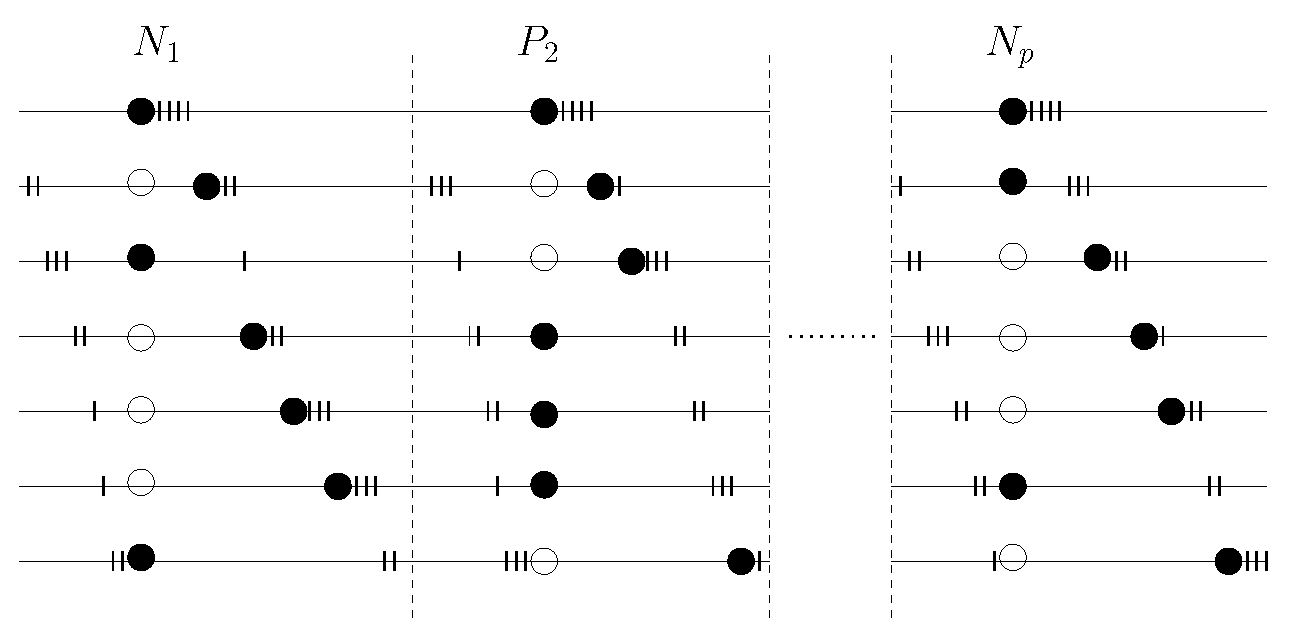
\includegraphics[angle=0,width=8cm]{generaldistribution.eps}}
\caption{$p$ elementary instances unified to form a single large instance.}\label{fig:generaldistribution}
\end{figure}

This defines a distribution on instances of alternation and redundancy
at most $\rho$ (as $4p=4\lfloor\rho/4\rfloor\leq\rho$), and of
signature at most $(k,n_1,\ldots,n_k)$.
%
Solving this instance implies to solve all the $p$ sub-instances.
Lemma~\ref{lem:elementproblem} gives a lower bound of
$(1/4)\sum_{i=2}^k\log (2n_i/p+1)+\sum_{i=2}^k{1/(2n_i{+}1)}-k{+}2$
comparisons on average for each of the $p$ sub problems, hence a lower
bound of
%
$$(p/4)
  \sum_{i=2}^k   \log(2n_i/p+1)  
               +p\left( \sum_{i=2}^k { 1 / (2n_i/p{+}1) }
                                 -k{+}2
                 \right)
,$$
%
which is $\Omega(\rho\sum_{i=1}^k\log (n_i/\rho))$.  \qed\end{proof}
%


\subsubsection{Application to Alternation}
\label{sec:appl-altern}


Indeed, among instances of same signature and alternation, it is
possible to prove a tight bound on the randomized complexity of the
intersection problem: by providing a difficult distribution of
instances and using the minimax principle, we prove a lower bound on
the complexity of any randomized algorithm solving the
problem~\cite{adaptiveIntersectionAndTThresholdProblems}.
%
\begin{theorem}[Alternation Lower Bound~\cite{adaptiveIntersectionAndTThresholdProblems}]\label{th:alternationLB}
For any $k{\geq} 2$, $0{<}n_1{\leq}\ldots{\leq}n_k$ and
$\delta{\in}\{4,\ldots,4n_1\}$,
%
and for any randomized algorithm $A_R$ for the intersection problem,
%
there is an instance of signature at most $(k,n_1,\ldots,n_k)$ and
alternation at most $\delta$,
%
such that $A_R$ performs $\Omega(\delta\sum_{i=1}^k\log(n_i/\delta))$
comparisons on average on it.
\end{theorem}
\begin{proof}
This is a simple application of Lemma~\ref{lem:generaldistribution}
(stated and proved in Section~\ref{sec:lowerbound})
and of the Yao-von Neumann principle \cite{vonneumann1944,sion58,yao}:
\begin{itemize}
\item Lemma~\ref{lem:generaldistribution} gives a distribution for
$\delta\in\{4,\ldots,4n_1\}$ on instances of
alternation {\em at most} $\delta$,
\item Then the Yao-von Neumann principle permits to deduce from this
distribution a lower bound on the worst case complexity of randomized
algorithms.  \qed\end{itemize}
\end{proof}

On the other hand, the simple deterministic algorithm of
Section~\ref{sec:alternation} reaches this lower bound.
%
As the class of deterministic algorithms is contained in the class of
randomized algorithms, this proves that the bound for the alternation
analysis is tight for randomized algorithms.
%



\subsubsection{Application to Redundancy}
\label{sec:appl-redund}





\begin{theorem}[Redundancy Lower Bound~\cite{optimalityOfRandomizedAlgorithmsForTheIntersectionProblem}]\label{th:standalonelowerbound} \label{th:redundancyLB}
For any $k\geq 2$, $0{<}n_1{\leq}\ldots{\leq}n_k$ and
$\rho\in\{4,\ldots,4n_1\}$, 
%
and for any randomized algorithm $A_R$ for the intersection problem,
%
there is an instance of signature at most $(k,n_1,\ldots,n_k)$, and
redundancy at most $\rho$,
%
such that $A_R$ performs $\Omega(\rho\sum_{i=1}^k\log(n_i/\rho))$
comparisons on average on it.
\end{theorem}

\begin{proof}
The proof is identical to the proof of Theorem~\ref{th:alternationLB},
as the instances generated by the proof are of alternation equal to
their redundancy.
%
This is a simple application of Lemma~\ref{lem:generaldistribution} and
of the Yao-von Neumann principle \cite{vonneumann1944,sion58,yao}:
\begin{itemize}
\item Lemma~\ref{lem:generaldistribution} gives a distribution for
$\rho\in\{4,\ldots,4n_1\}$ on instances of redundancy {\em at most}
$\rho$, 
\item Then the Yao-von Neumann principle permits to deduce from this
distribution a lower bound on the worst case complexity of randomized
algorithms.  \qed\end{itemize}
\end{proof}


This analysis is more precise than the lower bound previously
presented~\cite{adaptiveIntersectionAndTThresholdProblems}, where the
additive term in $-k$ was ignored, although it makes the lower bound
trivially negative for large values of the difficulty $\delta$.
%
Here the additive term is suppressed for $\min_i n_i\geq128$, and the
multiplicative factor between the lower bound and the upper bound is
reduced to $16$ instead of $64$.
%
This technique can be applied to the alternation analysis of the
intersection with the same result.
%
Note also that a multiplicative factor of $2$ in the gap comes from
the unbounded searches in the algorithm, and can be reduced using a
more complicated algorithm for the unbounded
search~\cite{anAlmostOptimalAlgorithmForUnboundedSearching}.



One could wonder how the lower bound evolves for redundancy values
larger than $4n_1$.
%
The following result shows that no instance with such redundancy can
exist.
%
\begin{lemma}\label{lem:rhoupperbound}
For any $k\geq 2$ and
$0{<}n_1{\leq}\ldots{\leq}n_k$, any instance of signature
$(k,n_1,\ldots,n_k)$ has redundancy $\rho$ at most $2n_1{+}1$.
\end{lemma}
\begin{proof}
First observe that there is always a partition-certificate of size
$2n_1+1$. Then that the redundancy of any partition-certificate is by
definition smaller than the size of the partition. Hence the result.
\qed\end{proof} 
%
Note that this does not contradict the result from
Lemma~\ref{lem:generaldistribution}, which defines a distribution of
instances of redundancy {\em at most} $4n_1$.

\subsection{Comparisons between the analysis}\label{sec:comparison}

The redundancy analysis is strictly finer than the alternation analysis:
%
some algorithms, optimal for the alternation analysis, are not optimal
anymore in the redundancy analysis (Theorem~\ref{th:finer}),
%
and any algorithm optimal in the redundancy analysis is optimal in the
alternation analysis (Theorem~\ref{th:strictlyfiner}).
%
So the {\tt Rand Intersection} algorithm is theoretically better than
its deterministic variant in the comparison model, and the redundancy
analysis permits a better analysis than the alternation analysis.

%
\begin{theorem}\label{th:finer}
For any $k\geq 2$, $0{<}n_1{\leq}\ldots{\leq}n_k$ and
$\rho\in\{4,\ldots,4n_1\}$, 
%
and for any deterministic algorithm for the intersection problem,
%
there is an instance of signature at most $(k,n_1,\ldots,n_k)$, and
redundancy at most $\rho$,
%
such that this algorithm performs $\Omega(k\rho\sum_i\log(n_i/k\rho))$
comparisons on it.
\end{theorem}
\begin{proof}
The proof uses the same decomposition than the proof of
Theorem~\ref{th:standalonelowerbound}, but uses an adversary argument
to obtain a deterministic lower bound.
%
Build $\delta={k\rho/3}$ sub-instances of signature
$(k,\lfloor{n_1/\delta}\rfloor,\ldots,\lfloor{n_k/\delta}\rfloor)$,
redundancy at most $3$, such that $x=A_1[1]$ is present in
roughly half of the other arrays, as in
Figure~\ref{fig:halffullsubinstance}.



On each sub-instance an adversary can force any deterministic algorithm
to perform a search in each of the arrays containing $x$, and in a
single array which does not contain $x$.
%
Then the deterministic algorithm performs
$(1/2)\sum_{i=2}^k\log{(n_i/\delta)}$ comparisons for each
sub-instance.
%
\begin{figure}
\hfill
\begin{minipage}{0.33\textwidth}
\centerline{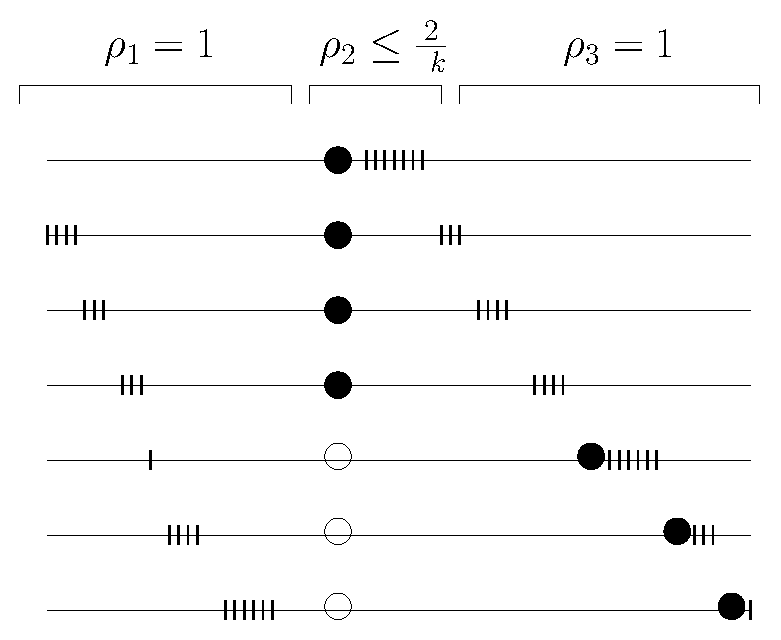
\includegraphics[angle=0,height=3.3cm]{halffullsubinstance.eps}}
\caption{Element $x$ is present in half of the arrays of the sub-instance.\label{fig:halffullsubinstance}
}
\end{minipage}
\hfill
\begin{minipage}{0.66\textwidth}
\centerline{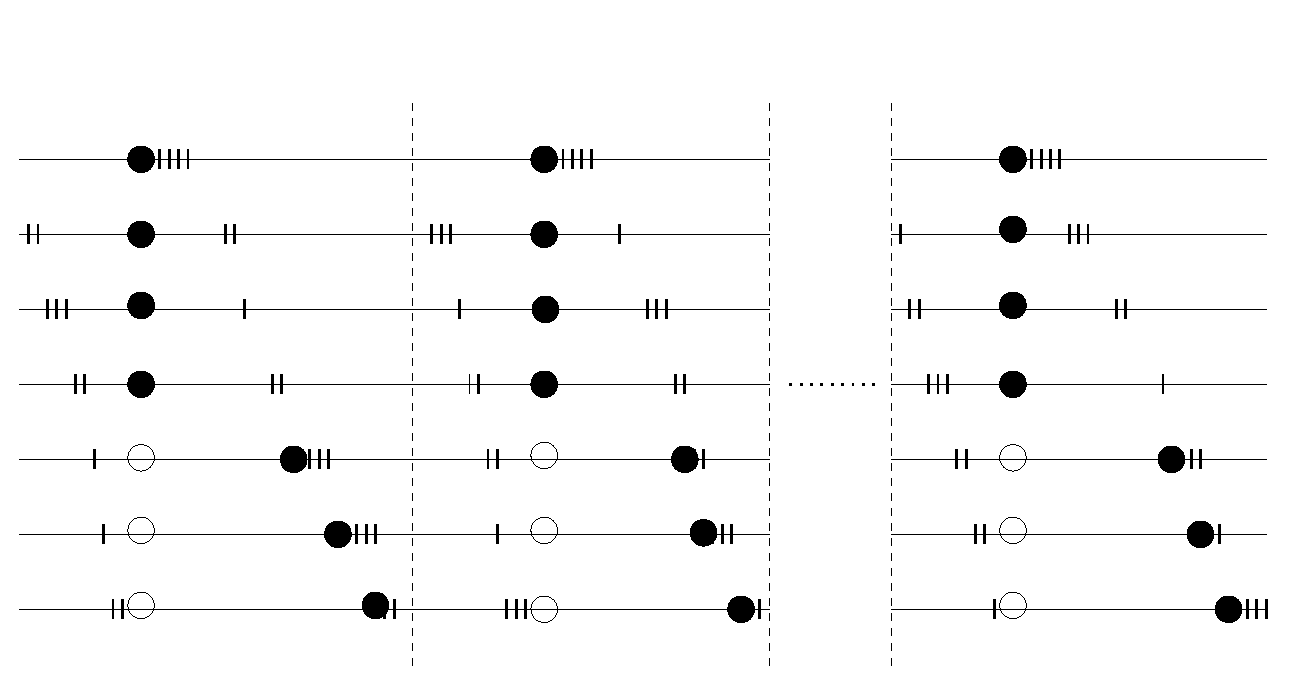
\includegraphics[angle=0,height=3.5cm]{halffullinstance.eps}}
\caption{The adversary performs several strategies in parallel, one
for each
sub-instance. \label{fig:halffullinstance}}\end{minipage}\hfill \hfill
\hfill \hfill
\end{figure}
%
In total over all sub-instances, the adversary can force any
deterministic algorithm to perform
${(\delta/2)}\sum_{i=2}^k\log{(n_i/\delta)}$ comparisons, i.e.
${(k\rho/4)}\sum_{i=2}^k\log{(n_i/k\rho)}$, which is
$\Omega({k\rho}\sum_{i=2}^k\log{(n_i/k\rho)})$.
\qed\end{proof}
%
As $x\log(n/x)$ is a function increasing with $x$,
$k\rho\sum_i\log(n_i/k\rho)$ is several times larger than the lower
bound $\rho\sum_i\log(n_i/\rho)$, hence no deterministic algorithm can
be optimal in the redundancy analysis.
%
\begin{theorem}\label{th:strictlyfiner}
Any algorithm optimal in the redundancy analysis is optimal in the
alternation analysis.
\end{theorem}
\begin{proof}
By definition of the redundancy $\rho$ and of the alternation $\delta$
of an instance, $\rho\leq\delta$.
%
So if an algorithm performs $O(\rho\sum \log{n_i/\rho})$
comparisons, it also performs $O(\delta\sum\log{n_i/\delta})$
comparisons.
%
Hence the result, as this is the lower bound in the alternation analysis.
\qed\end{proof}


This proves also that the measure of difficulty of
Demaine~\etal~\cite{dlm} is not comparable with the measure of
redundancy, as it is not comparable with the measure of
alternation~\cite[Section~2.3]{deterministicAlgorithmForTheTThresholdSetProblem}.
%
This means that the two measures are complementary, without being
redundant in any way, as it was for the alternation.
%
All those measures describe the difficulty of the instance:
\begin{itemize}
\item the {\em alternation}~\cite[Section~2.3]{deterministicAlgorithmForTheTThresholdSetProblem}
describes the number of key blocks of consecutive elements in the
instance;
\item the {\em gap cost}~\cite{dlm} describes the repartition of the
size of those blocks;
\item the {\em
redundancy}~\cite{optimalityOfRandomizedAlgorithmsForTheIntersectionProblem}
describes the difficulty to find each
block.
\end{itemize}
%
But only the {\em gap cost} and the {\em redundancy} matter, because the
alternation analysis is reduced to the redundancy analysis.



\section{Weighted $t$-Threshold Set}
\label{sec:t-threshold-set}



Conjunctive queries are well known. Indeed, most search engines
implement them.
% 
Given a list of labels (e.g.  keywords), the answer consists of all
the objects (e.g. webpage references) which are associated with all of
the labels.
%
Given an index such as described in the section above, solving a
conjunctive query composed of $\nbkeywords$ labels implies computing
the intersection of $\nbkeywords$ rows in a binary relation, which is
a well studied
problem~\cite{aFastSetIntersectionAlgorithmForSortedSequences,experimentalAnalysisOfAFastIntersectionAlgorithmForSortedSequences,dlm,dlmAlenex}


As an empty intersection can be an uninformative answer to a
conjunctive query, we should consider other approaches. 
%
Researchers in information retrieval suggest a number of ways to deal
with this problem.
%
For example, one can relax both queries and document index in a number
of different ways that are summarized by Bordogna and
Pasi~\cite{DBLP:conf/essir/BordognaP00}.
%
Barbay and Kenyon~\cite{adaptiveIntersectionAndTThresholdProblems}
proposed the adaptive algorithm to answer the query where for a given
parameter $\threshold$ the answer consists of the references matching
at least $\threshold$ of the $\nbkeywords$ labels composing the query.
%
Given an index such as described in the section above, solving this
new type of query implies computing the {\em threshold set} of 
$\nbkeywords$ rows in a binary relation, the set of objects associated
with at least $\threshold$ labels among the $\nbkeywords$ specified.

Barbay and Veraskouski
\cite{adaptiveAlgorithmsForWeightedQueriesOnWeightedBinaryRelationsAndLabeledTrees}
extended further this type of query to {\em weighted threshold}
queries, by considering
%
weighted queries $\Q:[\nblabels]\rightarrow\{0,\ldots,\maxWeightQ\}$,
where $\nblabels$ is the number of admissible keywords, and
%
weighted binary relations 
$\R:[\nblabels]\times[\nbobjects]\rightarrow\{0,\ldots,\maxWeightR\}$
~\footnote{By $[m]$ we denote $\{1, \ldots, m\}$ for any integer number $m$.}.
%
The {\em score} of an object $\objectx$ relative to a query $\Q$ on a
relation $\R$ is then defined as the linear combination of those
weights, i.e. $\score(\R,\Q,\objectx) = \sum_{\labelx \in
  [\nblabels]}{\Q(\labelx)\R(\labelx,\objectx)}$, that corresponds to
the notion of the {\em Retrieval Status Value} (or RSV) described by
Bordogna and Pasi~\cite{DBLP:conf/essir/BordognaP00}.
%
The answer to a query with parameter $\threshold$ is the set of
objects with score at least~$\threshold$: this definition matches the
original one from Barbay and Kenyon when each weight is either null or
unitary (the {\em unweighted} case).

We define the {\em alternation} of a weighted threshold set instance
as the size $\difficulty$ of the smallest possible
partition-certificate of the instance.
%
\begin{LONG}
  The alternation is related to the {\em non-deterministic} complexity
  of the instance, as it corresponds to the complexity of a
  non-deterministic algorithm which would produce the shortest
  partition-certificate of the instance.
\end{LONG}
% 
In the unweighted case (where all weights are unitary), if no object
match the query then the alternation is exactly the non-deterministic
complexity of the instance, i.e. the complexity of the best
non-deterministic algorithm checking the answer to the query.

\begin{figure}
  \centering
$$  \begin{array}[b]{cc|c|c|c|c|c|c|cccc|ccccc|cccccc|cccccccc}

    & 
    \multicolumn{7}{}  											                         &                    & & &
 1  &  2 &  3 &  4 &  5 &  6 &  7 & 8  &  9 &  10 &  11 & 12 &  13 &  14 & 15 & 16  & 17 & 18  &      &    
\\ \cline{3-8} \cline{11-28}


    \mbox{Music} & \rightarrow      
& 1                                & 8       & 10      & 12           & 15      & 17                 & & \rightarrow &
  1  &  . &  . &  . &  . &  . &  . & 1  &  . &  1 &  . &  1 &  . &  . &  1 &  . &  1 &  .  &   &    
\\ \cline{3-8}
    \mbox{Jazz} & \rightarrow
    & 2       & 4       & 6            & 9       & 11      & 13                                      & & \rightarrow &
  . & 1  &  . & 1  &  . & 1  &  . &  . & 1  &  . &  1 &  . &  1 &  . &  . &  . &  . &  . &     &    
\\ \cline{3-8}
    \mbox{Rock} & \rightarrow      
         & 3       & 5       & 7                                & 14      & 16      & 18             & & \rightarrow &
  . &  . & 1  &  . & 1  & .  & 1  &  . &  . &  . &  . &  . &  . &  1 &  . &  1 &  . &  1 &    
\\ \cline{3-8}
  \end{array}$$
  \begin{minipage}{.9\linewidth}
    \caption{ An example of how a conjunctive query composed 
      of three keywords corresponds to the
      intersection of the three corresponding sets.  
      % 
      The alternation of the instance is $\difficulty=4$, 
      the number of intervals of a partition certificate 
      where each interval has an empty intersection with at least one of the sets.
      % 
      Barbay and Kenyon's algorithm performs
      $7{\leq}\difficulty\nbkeywords{=}12$ searches (for the numbers
      $1,2,3,8,9,14,15$).  \label{fig:sequentialExample} }
  \end{minipage}
\end{figure}

Barbay and Kenyon~\cite{adaptiveIntersectionAndTThresholdProblems}
proved that any randomized algorithm performs
$\Omega(\difficulty\nbkeywords)$ searches in the worst case over
instances of difficulty $\difficulty$ on $\nbkeywords$ labels, and
proposed an optimal deterministic algorithm for the unweighted case on
sorted arrays.
%
We analyze the complexity of the algorithms in terms of search and
priority queue operations, where a priority queue operation is either an insertion or a
deletion from a priority queue, and where each search operation is a search for
the particular object in a data structure representing an ordered list
of objects.
%
We propose an optimal algorithm for the weighted case with any data
structure supporting the search for the insertion rank in an indexed
set:

\begin{theorem}\label{th:threshold-set}
  Consider a weighted binary relation
  $\R:[\nblabels]\times[\nbobjects]\rightarrow\{0,\ldots,\maxWeightR\}$,
  a weighted query
  $\Q:[\nblabels]\rightarrow\{0,\ldots,\maxWeightQ\}$, and a
  non-negative integer $\threshold$.
  % 
  There is an algorithm that computes the threshold set for $\Q$ on
  $\R$ with threshold-value of $\threshold$ in $\bigo(\difficulty\nbkeywords)$
  search and priority queue operations, where
  % 
  $\difficulty$ is the alternation of the instance and
  % 
  $\nbkeywords$ is the number of labels of positive weight in~$\Q$.
\end{theorem}

  \begin{algorithm}
    \centering
    \caption{Algorithm  answering Threshold Set queries }
    \label{alg:ThresholdOnBinRel}
    \begin{algorithmic}
      \STATE Set $\objectx$ to $-\infty$, 
      $\setNO$ and $\setYES$ to $\emptyset$
      and $\setMAYBE$ to the set of all labels of non-null weight;

      \STATE \idtt{Update}$(\objectx,\setYES,\setNO,\setMAYBE,\scoremin,\scoremax)$ 
      using Algorithm~\ref{alg:choiceBR};

      \WHILE{$\objectx<\infty$}

        \STATE Set $\labelx$ to the next label from $\setMAYBE$ in round
        robin order, and deduct $\maxWeightR\Q(\labelx)$ from
        $\scoremax$;

        \STATE Search for the insertion rank of $\objectx$ among the
        objects labeled $\labelx$;

        \IF{$\objectx$ is associated with a label $\labelx$}
          \STATE Move $\labelx$ from $\setMAYBE$ to $\setYES$;
          \STATE Add $\Q(\labelx)\R(\labelx,\objectx)$ to
          $\scoremin$ and $\scoremax$;
          \STATE {\bf if} {$\threshold\leq\scoremin$} 
                 {\bf then } Output $\objectx$;
        \ELSE    
          \STATE Move $\labelx$ from $\setMAYBE$ to $\setNO$;
        \ENDIF

        \IF{$\threshold \le \scoremin$ or $\threshold>\scoremax$}
           \STATE \idtt{Update}$(\objectx,\setYES,\setNO,\setMAYBE,\scoremin,\scoremax)$;
        \ENDIF

      \ENDWHILE
    \end{algorithmic}
  \end{algorithm}

  \begin{PROOF}
    \begin{proof}[of Theorem~\ref{th:threshold-set}]
      Consider the steps of Algorithm~\ref{alg:ThresholdOnBinRel}:
      given a query $\Q$ with $\nbkeywords$ positive weights and a
      threshold-value $\threshold$, the algorithm computes the set of
      objects scoring at least $\threshold$ for a weighted binary
      relation $\R$ associating objects with labels.

      Our algorithm goes through a number of phases. At each phase it
      considers one object $\objectx$, in increasing order, and bounds
      its score by an interval $[\scoremin,\scoremax]$.
  %
      The algorithm can decide whether $\objectx$ belongs to the
      result set through this interval and without computing the
      object's exact score
      ($\threshold\leq\scoremin\leq\score(\objectx)$).
  % 
      On the other hand, if for a given interval of consecutive
      objects there is a set of labels not associated with any of them
      with large total weight, this interval certifies that none of
      those objects belongs to the result set
      ($\score(\objectx)\leq\scoremax<\threshold$).
  % 
      The key issue of the algorithm is the choice of the values of
      $\objectx$ and of the labels to consider.

      This choice is described in Algorithm~\ref{alg:choiceBR}, which
      is based on the decomposition of the set of labels of positive
      weights in three disjoint sets: $\setYES$, $\setMAYBE$ and
      $\setNO$:
  %
      \begin{itemize}
      \item $\setYES$ corresponds to the labels already known to be
        associated with the current value of $\objectx$. It can be
        implemented as a simple set, for instance in an array.
      \item $\setMAYBE$ corresponds to the labels which could be
        associated with the current value of $\objectx$. It is
        implemented as a FIFO queue so that each label in it is
        considered equally often.
      \item $\setNO$ corresponds to the labels which are known not to
        be associated with the current value of $\objectx$. It is
        implemented as a priority queue of at most $\nbkeywords$
        elements, and the labels $\labelx$ it contains are ordered by
        the value of the first object larger than $\objectx$
        associated with label $\labelx$.
      \end{itemize}
  % 
      The values of the bounds $\scoremin$ and $\scoremax$ on the
      potential score of $\objectx$ are direct consequences of those
      definitions: $\scoremin$ depends on the weights of the labels in
      $\setYES$, i.e.
      $\scoremin=\sum_{\labelx\in\setYES}\Q(\labelx)\R(\labelx,\objectx)$;
      and $\scoremax$ adds the maximum potential weights of the labels
      in $\setMAYBE$ to $\scoremin$, i.e.
      $\scoremax=\scoremin+\sum_{\labelx\in\setMAYBE}\Q(\labelx)\maxWeightR$.

      To choose a new value for $\objectx$, the algorithm removes
      labels from the set $\setMAYBE$ till it reaches a critical
      weight, where removing any other label would make it impossible
      for an object matching only the labels of $\setMAYBE$ to score
      above the threshold.
  % 
      Then, the smallest object potentially in the result set
      corresponds to the first label of the priority queue
      implementing set $\setNO$.
 

      %%%%%%%%%%%%%%%%%% ADAPTIVE
      %%%%%%%%%%%%%%%%%% ANALYSIS %%%%%%%%%%%%%%%%%%%%%%%%%%%%%%%%%%%%%%%%%

      Consider a phase of the execution where the algorithm is
      processing an interval of the partition-certificate consisting
      of only one object $\objectx$.
      Algorithm~\ref{alg:ThresholdOnBinRel} performs at most
      $\nbkeywords$ iterations of the main loop to decide whether
      $\objectx$ has enough score or not without updating $\objectx$
      (through Algorithm~\ref{alg:choiceBR}). Once the decision about
      $\objectx$ is made, the algorithm updates $\objectx$ and moves
      to the next phase. Updating of $\objectx$ takes not more than
      $\nbkeywords$ loop iterations of Algorithm~\ref{alg:choiceBR}.
      Thus during each phase, the algorithm performs at most
      $\bigo(\nbkeywords)$ search and priority queue operations.

      Consider a phase corresponding to the interval of the
      partition-certificate that does not have any objects with enough
      score and a subset $S$ of labels that are not associated with
      any of the objects in this interval.
      Algorithm~\ref{alg:ThresholdOnBinRel} may update $\objectx$ more
      than once during the same phase. We prove the upper bound on the
      number of operations through considering the way the algorithm
      moves labels from one set to another.
  
      The only way Algorithm~\ref{alg:ThresholdOnBinRel} moves labels
      is from set $\setMAYBE$ to either set $\setYES$ or set $\setNO$.
      Algorithm~\ref{alg:choiceBR}, on the other hand, move labels
      from $\setYES$ to $\setMAYBE$, from $\setMAYBE$ to $\setNO$, and
      from $\setNO$ to $\setYES$ in this order. As it cannot move
      labels that are in $S$ to $\setYES$, the algorithm has the only
      possible loop $\setMAYBE \longrightarrow \setNO \longrightarrow
      \setYES \longrightarrow \setMAYBE$ for these labels.
  
      However, the algorithm does not move any labels from $S$ that it
      already moved to $\setNO$ during the processing of the same
      interval, because the label's successor is out of the current
      interval and cannot be processed in the current phase. While the
      algorithm retrieves labels from set $\setMAYBE$ in round-robin
      order, it cannot retrieve any label from set $\setMAYBE$ for the
      second time until all the labels from subset $S$ appear in set
      $\setNO$, which effectively means that the next element
      $\objectx$ will be outside of the interval and the algorithm
      proceeds to the new phase. While it takes a constant time for
      the algorithm to move each label from set $\setMAYBE$ back to
      set $\setMAYBE$, it needs $\bigo(\nbkeywords)$ search and
      priority queue operations to complete this phase.
  
      As the algorithm spends $\bigo(\nbkeywords)$ to complete any
      phase, and any instance has $\difficulty$ intervals that
      correspond to $\difficulty$ phases, the total complexity of the
      algorithm is $\bigo(\difficulty \nbkeywords)$.  \qed
    \end{proof}
  \end{PROOF}
      \begin{algorithm}
        \begin{algorithmic}
          \caption{\idtt{Update}$(\objectx,\setYES,\setNO,\setMAYBE,\scoremin,\scoremax)$}
          \label{alg:choiceBR}
 
          \STATE Add all the labels from $\setYES$ to the set
          $\setMAYBE$ and set $\scoremax$ to
          $\sum_{\labelx\in\setMAYBE}\Q(\labelx)\maxWeightR$; \STATE
          Choose a label $\labelx$ in round-robin order from
          $\setMAYBE$;

          \WHILE{$\scoremax-\Q(\labelx)\maxWeightR \ge \threshold$}
          \STATE Deduct $\Q(\labelx)\maxWeightR$ from $\scoremax$, and
          move $\labelx$ from $\setMAYBE$ to $\setNO$; \STATE Choose a
          label $\labelx$ in round-robin order from $\setMAYBE$;
          \ENDWHILE

          \STATE Find the subset $S\subset\setNO$ of labels $\labelx$
          such that the successor of $\objectx$ among the objects
          labeled $\labelx$ is minimal;

          \STATE Move all the labels of $S$ from $\setNO$ to
          $\setYES$, and set $\scoremin$ to
          $\sum_{\labelx\in\setYES}\Q(\labelx)\R(\labelx,\objectx)$;
      
          \STATE Update $\objectx$ to its successor among the objects
          labeled $\labelx$, for any label in $\setYES$;
        \end{algorithmic}
      \end{algorithm}

  Note that $\nbkeywords$ is the number of labels with a positive weight.
  % 
  If the binary relation is implemented by postings lists, and the
  priority queue is implemented using a heap, the complexity of the
  algorithm is $\bigo ( \difficulty \nbkeywords \lg (n / (\difficulty
  \nbkeywords)) + \difficulty \nbkeywords \lg {\nbkeywords } )$, where
  $n$ is the sum of the sizes of all postings lists and $\nbkeywords$
  is the maximum size of the priority queue.
  % 
  If the binary relation is implemented using
  Barbay~\etal's~\cite{weightedQueriesOnBinaryRelationsAndMultiLabeledTrees}
  succinct encoding and the priority queue is implemented using
  Andersson and
  Thorup's~\cite{tighterWorstCaseBoundsOnDynamicSearchingAndPriorityQueues}
  structure, the complexity of the algorithm is
  $\bigo(\difficulty\nbkeywords\lg\lg\nblabels +
  \difficulty\nbkeywords(\lg\lg\nbkeywords)^2)$ in the RAM model with
  word size $\Theta(\lg\max\{\nblabels,\nbobjects\})$.













\section{Perspectives}
\label{sec:perspectives}


The $t$-threshold set and opt-threshold set
problems~\cite{deterministicAlgorithmForTheTThresholdSetProblem} are
natural generalizations of the intersection problem, which could be
useful in indexed search engines.
%
The redundancy seems to be important in the complexity of these
problems as well, but a proper measure is harder to define in this
context.
%
As similar techniques are applied to solve queries on semi-structured
documents~\cite{indexTreesForDescendantTreeQueriesInTheComparisonModel},
the redundancy could be useful in this domain too, but the definition
of the proper measure of difficulty is even more evasive in this
context.
%
More generally, the set operations are combined in practice in a
recursive way, forming Union/Intersection trees.
%
Farzan~\etal~\cite{worstCaseOptimalUnionIntersectionExpressionEvaluation}
studied the non-adaptive complexity of the evaluation of such
expressions: the adaptive analysis of such a problem is still an open
problem.


Demaine~\etal~\cite{dlmAlenex} performed experimental measurements of
the performance of various deterministic algorithms for the
intersection on their own data using some queries provided by
\texttt{Google}.
%
We performed similar measurements for the deterministic and randomized
version of our algorithm, using the same queries and a larger set of
data, also provided by Google.
%
The results are quite disappointing, as the randomized version of the
algorithm does not perform better than the deterministic one in term
of the number of comparisons or searches, and much worst in term
of runtime.
%
The fact that the number of comparisons and the number of
searches are roughly the same indicates that most instances of
this data set either have a redundancy close to the alternation,
because the elements searched are in many of the arrays, or are so
easy that both algorithms perform equally well on it.
%
The fact that the runtime is worse is probably linked to the
performance of prediction heuristics in the hardware: a deterministic
algorithm is easier to predict than a randomized one.
%
It would be interesting to see if those negative results still holds
for queries with more keywords and on some data sets such as those
from relational databases, which can exhibit more correlation between
keywords.



While we restricted our definition of the intersection problem to set
of arrays and analyzed it in the comparison model, it makes sense to
consider other structures for sorted sets, especially in the context
of cached or swapped memory, or succinct encodings of
dictionaries.
%
The {\em hierarchical memory}~\cite{cacheObliviousAlgorithms} seems
promising for this kind of application, and
Bender~\etal~\cite{exponentialStructuresForEfficientCacheObliviousAlgorithms}
proposed a data structure and a {\em cache oblivious} algorithm to
perform unbounded searches (implemented as finger searches).
%
Our algorithm can easily be adapted to this model, to perform
$O(\rho\sum(\log_B(n_i/\rho)+\log^*(n_i/\rho)))$ I/O transfers at the
level of cache size~$B$.


\def\select{\hbox{\tt select}}
\def\rank{\hbox{\tt rank}}
%
In most of the intersection algorithms, the interactions with each set
are limited to accessing an element given its rank ($\select$ operator)
and searching for the insertion rank of an element in it ($\rank$
operator): those algorithms can be used with any set implementation
which provides those operators.
%
For instance, using sorted arrays such as in this paper, the $\select$
operator takes constant time while the $\rank$ operator takes
logarithmic time in the size of the set.
%
While the results of this paper are optimal in the comparison model,
it is not necessary optimal in more general models: the computational
complexity of the search operators is a trade-off with the size of the
encoding of the set.
%
For instance, consider a set of $n$ elements from a universe of size
$m$:
Raman~\etal~\cite{succinctIndexableDictionariesWithApplicationsToEncodingKAryTreesAndMultisets}
propose a succinct encoding of Fully Indexable Dictionaries using
$\log {m \choose n} + o(m)$ bits to provide $\select$ and $\rank$
operators in constant time.
%
On the other side of the time/space trade-off, Beame and
Fish~\cite{optimalBoundsForThePredecessorProblem} proposed a more
compact encoding, using $O(n)$ words of $\log m$ bits to provide
$\select$ and $\rank$ operators in time $O(\sqrt{ \log n / \log \log
  n})$.
%
Encoding the sets using any of those schema would tremendously improve
the computational complexity of the intersection, at a small cost in
space, which could result in much faster search engines.




%%% Local Variables: 
%%% mode: latex
%%% TeX-master: "adaptiveAnalysisOfAlgorithm"
%%% End: 
